
\begin{recipe}
    [% 
        preparationtime = {\unit[30]{min}},
        bakingtime = {\unit[1~\nicefrac{1}{2}]{h}}
    ]
    {Beetroot carpaccio}

    \introduction{%
        Easy salad, perfect for hot summer garden party or as a starter before fancy dinner.
    }

    \setRecipeLengths{
        ingredientswidth=5cm
    }
    \ingredients[9]{%
        4 & Beetroots (elongated ones are the best) \\
        & Feta cheese \textbf{or} \\
        & goat cheese \\
        & Balsamic vinegar \\
        & Olive oil \\
        & Rocket \\
        & Pumpkin seed \textbf{or} \\
        & pistachio
    }

    \preparation{%
        \step Cover washed raw beetroot in aluminium foil.
        Bake till tender (around 1-1~\nicefrac{1}{2}h)
        \step Slices thinly.
        Sprinkle with olive oil, black pepper and balsamic vinegar.
        \step Scatter cheese, rocket and seeds.
        Add extra olive oil and balsamic vinegar.
        
        \begin{figure}[h]
            \centering
            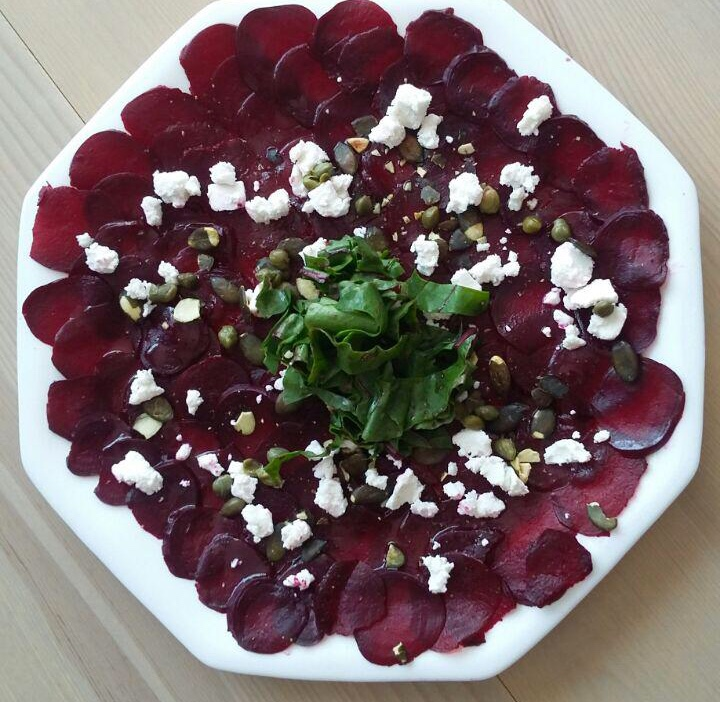
\includegraphics[width=6cm]{pic/beetroot_carpaccio}
        \end{figure}        
    }

    \hint
    {%
        It's a lot of faff to bake just a few beetroots.
        Instead, bake them when baking something else.
        Since they're covered in foil, fragrances shouldn't permeate.
    }

\end{recipe}